% Created by tikzDevice version 0.12.6 on 2023-12-10 22:55:56
% !TEX encoding = UTF-8 Unicode
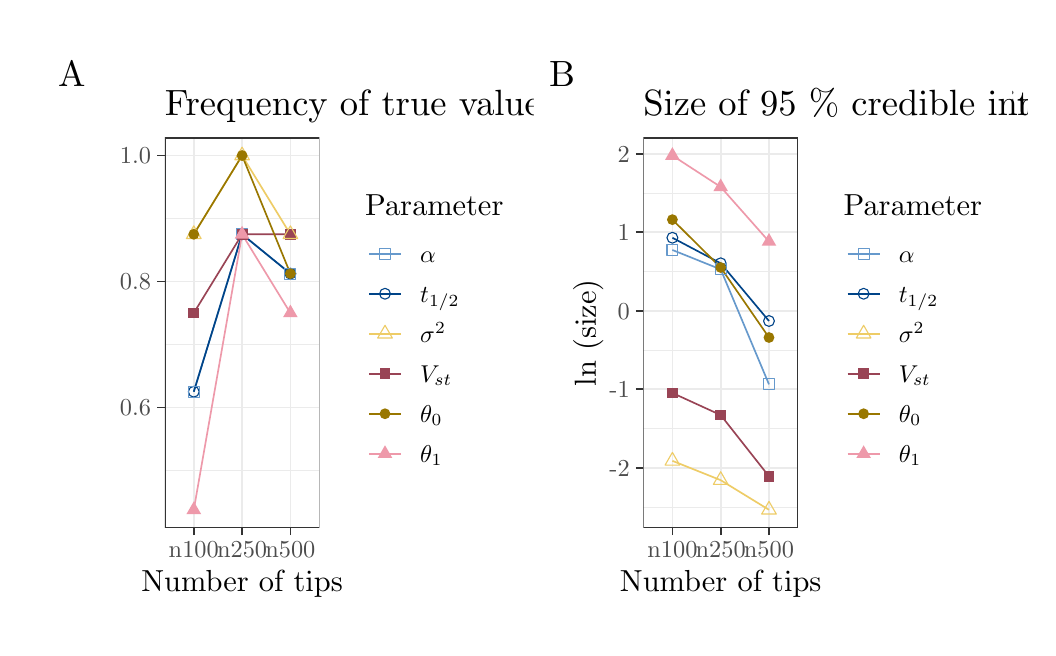
\begin{tikzpicture}[x=1pt,y=1pt]
\definecolor{fillColor}{RGB}{255,255,255}
\path[use as bounding box,fill=fillColor,fill opacity=0.00] (0,0) rectangle (361.35,216.81);
\begin{scope}
\path[clip] (  0.00,  0.00) rectangle (361.35,216.81);
\definecolor{drawColor}{RGB}{255,255,255}
\definecolor{fillColor}{RGB}{255,255,255}

\path[draw=drawColor,line width= 0.6pt,line join=round,line cap=round,fill=fillColor] (  0.00,  0.00) rectangle (361.35,216.81);
\end{scope}
\begin{scope}
\path[clip] (  5.50,  5.50) rectangle (182.91,211.31);
\definecolor{drawColor}{RGB}{255,255,255}
\definecolor{fillColor}{RGB}{255,255,255}

\path[draw=drawColor,line width= 0.6pt,line join=round,line cap=round,fill=fillColor] (  5.50,  5.50) rectangle (182.91,211.31);
\end{scope}
\begin{scope}
\path[clip] ( 49.55, 36.19) rectangle (105.40,177.00);
\definecolor{fillColor}{RGB}{255,255,255}

\path[fill=fillColor] ( 49.55, 36.19) rectangle (105.40,177.00);
\definecolor{drawColor}{gray}{0.92}

\path[draw=drawColor,line width= 0.3pt,line join=round] ( 49.55, 56.81) --
	(105.40, 56.81);

\path[draw=drawColor,line width= 0.3pt,line join=round] ( 49.55,102.32) --
	(105.40,102.32);

\path[draw=drawColor,line width= 0.3pt,line join=round] ( 49.55,147.84) --
	(105.40,147.84);

\path[draw=drawColor,line width= 0.6pt,line join=round] ( 49.55, 79.57) --
	(105.40, 79.57);

\path[draw=drawColor,line width= 0.6pt,line join=round] ( 49.55,125.08) --
	(105.40,125.08);

\path[draw=drawColor,line width= 0.6pt,line join=round] ( 49.55,170.60) --
	(105.40,170.60);

\path[draw=drawColor,line width= 0.6pt,line join=round] ( 60.02, 36.19) --
	( 60.02,177.00);

\path[draw=drawColor,line width= 0.6pt,line join=round] ( 77.48, 36.19) --
	( 77.48,177.00);

\path[draw=drawColor,line width= 0.6pt,line join=round] ( 94.93, 36.19) --
	( 94.93,177.00);
\definecolor{drawColor}{RGB}{102,153,204}

\path[draw=drawColor,line width= 0.6pt,line join=round] ( 60.02, 85.26) --
	( 77.48,142.15) --
	( 94.93,127.93);
\definecolor{drawColor}{RGB}{0,68,136}

\path[draw=drawColor,line width= 0.6pt,line join=round] ( 60.02, 85.26) --
	( 77.48,142.15) --
	( 94.93,127.93);
\definecolor{drawColor}{RGB}{238,204,102}

\path[draw=drawColor,line width= 0.6pt,line join=round] ( 60.02,142.15) --
	( 77.48,170.60) --
	( 94.93,142.15);
\definecolor{drawColor}{RGB}{153,68,85}

\path[draw=drawColor,line width= 0.6pt,line join=round] ( 60.02,113.70) --
	( 77.48,142.15) --
	( 94.93,142.15);
\definecolor{drawColor}{RGB}{153,119,0}

\path[draw=drawColor,line width= 0.6pt,line join=round] ( 60.02,142.15) --
	( 77.48,170.60) --
	( 94.93,127.93);
\definecolor{drawColor}{RGB}{238,153,170}

\path[draw=drawColor,line width= 0.6pt,line join=round] ( 60.02, 42.59) --
	( 77.48,142.15) --
	( 94.93,113.70);
\definecolor{drawColor}{RGB}{0,68,136}

\path[draw=drawColor,line width= 0.4pt,line join=round,line cap=round] ( 60.02, 85.26) circle (  1.96);
\definecolor{drawColor}{RGB}{102,153,204}

\path[draw=drawColor,line width= 0.4pt,line join=round,line cap=round] ( 58.06, 83.29) rectangle ( 61.99, 87.22);
\definecolor{fillColor}{RGB}{153,68,85}

\path[fill=fillColor] ( 58.06,111.74) --
	( 61.99,111.74) --
	( 61.99,115.66) --
	( 58.06,115.66) --
	cycle;
\definecolor{drawColor}{RGB}{238,204,102}

\path[draw=drawColor,line width= 0.4pt,line join=round,line cap=round] ( 60.02,145.20) --
	( 62.67,140.62) --
	( 57.38,140.62) --
	cycle;
\definecolor{fillColor}{RGB}{153,119,0}

\path[fill=fillColor] ( 60.02,142.15) circle (  1.96);
\definecolor{fillColor}{RGB}{238,153,170}

\path[fill=fillColor] ( 60.02, 45.64) --
	( 62.67, 41.06) --
	( 57.38, 41.06) --
	cycle;
\definecolor{drawColor}{RGB}{0,68,136}

\path[draw=drawColor,line width= 0.4pt,line join=round,line cap=round] ( 77.48,142.15) circle (  1.96);
\definecolor{drawColor}{RGB}{102,153,204}

\path[draw=drawColor,line width= 0.4pt,line join=round,line cap=round] ( 75.51,140.19) rectangle ( 79.44,144.11);
\definecolor{fillColor}{RGB}{153,68,85}

\path[fill=fillColor] ( 75.51,140.19) --
	( 79.44,140.19) --
	( 79.44,144.11) --
	( 75.51,144.11) --
	cycle;
\definecolor{drawColor}{RGB}{238,204,102}

\path[draw=drawColor,line width= 0.4pt,line join=round,line cap=round] ( 77.48,173.65) --
	( 80.12,169.07) --
	( 74.83,169.07) --
	cycle;
\definecolor{fillColor}{RGB}{153,119,0}

\path[fill=fillColor] ( 77.48,170.60) circle (  1.96);
\definecolor{fillColor}{RGB}{238,153,170}

\path[fill=fillColor] ( 77.48,145.20) --
	( 80.12,140.62) --
	( 74.83,140.62) --
	cycle;
\definecolor{drawColor}{RGB}{0,68,136}

\path[draw=drawColor,line width= 0.4pt,line join=round,line cap=round] ( 94.93,127.93) circle (  1.96);
\definecolor{drawColor}{RGB}{102,153,204}

\path[draw=drawColor,line width= 0.4pt,line join=round,line cap=round] ( 92.96,125.96) rectangle ( 96.89,129.89);
\definecolor{fillColor}{RGB}{153,68,85}

\path[fill=fillColor] ( 92.96,140.19) --
	( 96.89,140.19) --
	( 96.89,144.11) --
	( 92.96,144.11) --
	cycle;
\definecolor{drawColor}{RGB}{238,204,102}

\path[draw=drawColor,line width= 0.4pt,line join=round,line cap=round] ( 94.93,145.20) --
	( 97.57,140.62) --
	( 92.28,140.62) --
	cycle;
\definecolor{fillColor}{RGB}{153,119,0}

\path[fill=fillColor] ( 94.93,127.93) circle (  1.96);
\definecolor{fillColor}{RGB}{238,153,170}

\path[fill=fillColor] ( 94.93,116.75) --
	( 97.57,112.18) --
	( 92.28,112.18) --
	cycle;
\definecolor{drawColor}{gray}{0.20}

\path[draw=drawColor,line width= 0.6pt,line join=round,line cap=round] ( 49.55, 36.19) rectangle (105.40,177.00);
\end{scope}
\begin{scope}
\path[clip] (  0.00,  0.00) rectangle (361.35,216.81);
\definecolor{drawColor}{gray}{0.30}

\node[text=drawColor,anchor=base east,inner sep=0pt, outer sep=0pt, scale=  0.88] at ( 44.60, 76.54) {0.6};

\node[text=drawColor,anchor=base east,inner sep=0pt, outer sep=0pt, scale=  0.88] at ( 44.60,122.05) {0.8};

\node[text=drawColor,anchor=base east,inner sep=0pt, outer sep=0pt, scale=  0.88] at ( 44.60,167.56) {1.0};
\end{scope}
\begin{scope}
\path[clip] (  0.00,  0.00) rectangle (361.35,216.81);
\definecolor{drawColor}{gray}{0.20}

\path[draw=drawColor,line width= 0.6pt,line join=round] ( 46.80, 79.57) --
	( 49.55, 79.57);

\path[draw=drawColor,line width= 0.6pt,line join=round] ( 46.80,125.08) --
	( 49.55,125.08);

\path[draw=drawColor,line width= 0.6pt,line join=round] ( 46.80,170.60) --
	( 49.55,170.60);
\end{scope}
\begin{scope}
\path[clip] (  0.00,  0.00) rectangle (361.35,216.81);
\definecolor{drawColor}{gray}{0.20}

\path[draw=drawColor,line width= 0.6pt,line join=round] ( 60.02, 33.44) --
	( 60.02, 36.19);

\path[draw=drawColor,line width= 0.6pt,line join=round] ( 77.48, 33.44) --
	( 77.48, 36.19);

\path[draw=drawColor,line width= 0.6pt,line join=round] ( 94.93, 33.44) --
	( 94.93, 36.19);
\end{scope}
\begin{scope}
\path[clip] (  0.00,  0.00) rectangle (361.35,216.81);
\definecolor{drawColor}{gray}{0.30}

\node[text=drawColor,anchor=base,inner sep=0pt, outer sep=0pt, scale=  0.88] at ( 60.02, 25.18) {n100};

\node[text=drawColor,anchor=base,inner sep=0pt, outer sep=0pt, scale=  0.88] at ( 77.48, 25.18) {n250};

\node[text=drawColor,anchor=base,inner sep=0pt, outer sep=0pt, scale=  0.88] at ( 94.93, 25.18) {n500};
\end{scope}
\begin{scope}
\path[clip] (  0.00,  0.00) rectangle (361.35,216.81);
\definecolor{drawColor}{RGB}{0,0,0}

\node[text=drawColor,anchor=base,inner sep=0pt, outer sep=0pt, scale=  1.10] at ( 77.48, 13.14) {Number of tips};
\end{scope}
\begin{scope}
\path[clip] (  0.00,  0.00) rectangle (361.35,216.81);
\definecolor{fillColor}{RGB}{255,255,255}

\path[fill=fillColor] (116.40, 50.12) rectangle (177.41,163.06);
\end{scope}
\begin{scope}
\path[clip] (  0.00,  0.00) rectangle (361.35,216.81);
\definecolor{drawColor}{RGB}{0,0,0}

\node[text=drawColor,anchor=base west,inner sep=0pt, outer sep=0pt, scale=  1.10] at (121.90,148.91) {Parameter};
\end{scope}
\begin{scope}
\path[clip] (  0.00,  0.00) rectangle (361.35,216.81);
\definecolor{fillColor}{RGB}{255,255,255}

\path[fill=fillColor] (121.90,127.89) rectangle (136.35,142.35);
\end{scope}
\begin{scope}
\path[clip] (  0.00,  0.00) rectangle (361.35,216.81);
\definecolor{drawColor}{RGB}{102,153,204}

\path[draw=drawColor,line width= 0.6pt,line join=round] (123.34,135.12) -- (134.91,135.12);
\end{scope}
\begin{scope}
\path[clip] (  0.00,  0.00) rectangle (361.35,216.81);
\definecolor{drawColor}{RGB}{102,153,204}

\path[draw=drawColor,line width= 0.4pt,line join=round,line cap=round] (127.16,133.16) rectangle (131.09,137.08);
\end{scope}
\begin{scope}
\path[clip] (  0.00,  0.00) rectangle (361.35,216.81);
\definecolor{fillColor}{RGB}{255,255,255}

\path[fill=fillColor] (121.90,113.44) rectangle (136.35,127.89);
\end{scope}
\begin{scope}
\path[clip] (  0.00,  0.00) rectangle (361.35,216.81);
\definecolor{drawColor}{RGB}{0,68,136}

\path[draw=drawColor,line width= 0.6pt,line join=round] (123.34,120.66) -- (134.91,120.66);
\end{scope}
\begin{scope}
\path[clip] (  0.00,  0.00) rectangle (361.35,216.81);
\definecolor{drawColor}{RGB}{0,68,136}

\path[draw=drawColor,line width= 0.4pt,line join=round,line cap=round] (129.12,120.66) circle (  1.96);
\end{scope}
\begin{scope}
\path[clip] (  0.00,  0.00) rectangle (361.35,216.81);
\definecolor{fillColor}{RGB}{255,255,255}

\path[fill=fillColor] (121.90, 98.98) rectangle (136.35,113.44);
\end{scope}
\begin{scope}
\path[clip] (  0.00,  0.00) rectangle (361.35,216.81);
\definecolor{drawColor}{RGB}{238,204,102}

\path[draw=drawColor,line width= 0.6pt,line join=round] (123.34,106.21) -- (134.91,106.21);
\end{scope}
\begin{scope}
\path[clip] (  0.00,  0.00) rectangle (361.35,216.81);
\definecolor{drawColor}{RGB}{238,204,102}

\path[draw=drawColor,line width= 0.4pt,line join=round,line cap=round] (129.12,109.26) --
	(131.77,104.68) --
	(126.48,104.68) --
	cycle;
\end{scope}
\begin{scope}
\path[clip] (  0.00,  0.00) rectangle (361.35,216.81);
\definecolor{fillColor}{RGB}{255,255,255}

\path[fill=fillColor] (121.90, 84.53) rectangle (136.35, 98.98);
\end{scope}
\begin{scope}
\path[clip] (  0.00,  0.00) rectangle (361.35,216.81);
\definecolor{drawColor}{RGB}{153,68,85}

\path[draw=drawColor,line width= 0.6pt,line join=round] (123.34, 91.76) -- (134.91, 91.76);
\end{scope}
\begin{scope}
\path[clip] (  0.00,  0.00) rectangle (361.35,216.81);
\definecolor{fillColor}{RGB}{153,68,85}

\path[fill=fillColor] (127.16, 89.79) --
	(131.09, 89.79) --
	(131.09, 93.72) --
	(127.16, 93.72) --
	cycle;
\end{scope}
\begin{scope}
\path[clip] (  0.00,  0.00) rectangle (361.35,216.81);
\definecolor{fillColor}{RGB}{255,255,255}

\path[fill=fillColor] (121.90, 70.08) rectangle (136.35, 84.53);
\end{scope}
\begin{scope}
\path[clip] (  0.00,  0.00) rectangle (361.35,216.81);
\definecolor{drawColor}{RGB}{153,119,0}

\path[draw=drawColor,line width= 0.6pt,line join=round] (123.34, 77.30) -- (134.91, 77.30);
\end{scope}
\begin{scope}
\path[clip] (  0.00,  0.00) rectangle (361.35,216.81);
\definecolor{fillColor}{RGB}{153,119,0}

\path[fill=fillColor] (129.12, 77.30) circle (  1.96);
\end{scope}
\begin{scope}
\path[clip] (  0.00,  0.00) rectangle (361.35,216.81);
\definecolor{fillColor}{RGB}{255,255,255}

\path[fill=fillColor] (121.90, 55.62) rectangle (136.35, 70.08);
\end{scope}
\begin{scope}
\path[clip] (  0.00,  0.00) rectangle (361.35,216.81);
\definecolor{drawColor}{RGB}{238,153,170}

\path[draw=drawColor,line width= 0.6pt,line join=round] (123.34, 62.85) -- (134.91, 62.85);
\end{scope}
\begin{scope}
\path[clip] (  0.00,  0.00) rectangle (361.35,216.81);
\definecolor{fillColor}{RGB}{238,153,170}

\path[fill=fillColor] (129.12, 65.90) --
	(131.77, 61.32) --
	(126.48, 61.32) --
	cycle;
\end{scope}
\begin{scope}
\path[clip] (  0.00,  0.00) rectangle (361.35,216.81);
\definecolor{drawColor}{RGB}{0,0,0}

\node[text=drawColor,anchor=base west,inner sep=0pt, outer sep=0pt, scale=  0.88] at (141.85,132.09) {$\alpha$};
\end{scope}
\begin{scope}
\path[clip] (  0.00,  0.00) rectangle (361.35,216.81);
\definecolor{drawColor}{RGB}{0,0,0}

\node[text=drawColor,anchor=base west,inner sep=0pt, outer sep=0pt, scale=  0.88] at (141.85,117.63) {$t_{1/2}$};
\end{scope}
\begin{scope}
\path[clip] (  0.00,  0.00) rectangle (361.35,216.81);
\definecolor{drawColor}{RGB}{0,0,0}

\node[text=drawColor,anchor=base west,inner sep=0pt, outer sep=0pt, scale=  0.88] at (141.85,103.18) {$\sigma^2$};
\end{scope}
\begin{scope}
\path[clip] (  0.00,  0.00) rectangle (361.35,216.81);
\definecolor{drawColor}{RGB}{0,0,0}

\node[text=drawColor,anchor=base west,inner sep=0pt, outer sep=0pt, scale=  0.88] at (141.85, 88.73) {$V_{st}$};
\end{scope}
\begin{scope}
\path[clip] (  0.00,  0.00) rectangle (361.35,216.81);
\definecolor{drawColor}{RGB}{0,0,0}

\node[text=drawColor,anchor=base west,inner sep=0pt, outer sep=0pt, scale=  0.88] at (141.85, 74.27) {$\theta_0$};
\end{scope}
\begin{scope}
\path[clip] (  0.00,  0.00) rectangle (361.35,216.81);
\definecolor{drawColor}{RGB}{0,0,0}

\node[text=drawColor,anchor=base west,inner sep=0pt, outer sep=0pt, scale=  0.88] at (141.85, 59.82) {$\theta_1$};
\end{scope}
\begin{scope}
\path[clip] (  0.00,  0.00) rectangle (361.35,216.81);
\definecolor{drawColor}{RGB}{0,0,0}

\node[text=drawColor,anchor=base west,inner sep=0pt, outer sep=0pt, scale=  1.32] at ( 49.55,185.06) {Frequency of true values falling within $\newline 95\%$ credible interval};
\end{scope}
\begin{scope}
\path[clip] (  0.00,  0.00) rectangle (361.35,216.81);
\definecolor{drawColor}{RGB}{0,0,0}

\node[text=drawColor,anchor=base,inner sep=0pt, outer sep=0pt, scale=  1.32] at ( 15.95,195.44) {A};
\end{scope}
\begin{scope}
\path[clip] (182.91,  5.50) rectangle (355.85,211.31);
\definecolor{drawColor}{RGB}{255,255,255}
\definecolor{fillColor}{RGB}{255,255,255}

\path[draw=drawColor,line width= 0.6pt,line join=round,line cap=round,fill=fillColor] (182.91,  5.50) rectangle (355.85,211.31);
\end{scope}
\begin{scope}
\path[clip] (222.50, 36.19) rectangle (278.34,177.00);
\definecolor{fillColor}{RGB}{255,255,255}

\path[fill=fillColor] (222.50, 36.19) rectangle (278.34,177.00);
\definecolor{drawColor}{gray}{0.92}

\path[draw=drawColor,line width= 0.3pt,line join=round] (222.50, 43.62) --
	(278.34, 43.62);

\path[draw=drawColor,line width= 0.3pt,line join=round] (222.50, 71.99) --
	(278.34, 71.99);

\path[draw=drawColor,line width= 0.3pt,line join=round] (222.50,100.35) --
	(278.34,100.35);

\path[draw=drawColor,line width= 0.3pt,line join=round] (222.50,128.72) --
	(278.34,128.72);

\path[draw=drawColor,line width= 0.3pt,line join=round] (222.50,157.08) --
	(278.34,157.08);

\path[draw=drawColor,line width= 0.6pt,line join=round] (222.50, 57.81) --
	(278.34, 57.81);

\path[draw=drawColor,line width= 0.6pt,line join=round] (222.50, 86.17) --
	(278.34, 86.17);

\path[draw=drawColor,line width= 0.6pt,line join=round] (222.50,114.54) --
	(278.34,114.54);

\path[draw=drawColor,line width= 0.6pt,line join=round] (222.50,142.90) --
	(278.34,142.90);

\path[draw=drawColor,line width= 0.6pt,line join=round] (222.50,171.26) --
	(278.34,171.26);

\path[draw=drawColor,line width= 0.6pt,line join=round] (232.97, 36.19) --
	(232.97,177.00);

\path[draw=drawColor,line width= 0.6pt,line join=round] (250.42, 36.19) --
	(250.42,177.00);

\path[draw=drawColor,line width= 0.6pt,line join=round] (267.87, 36.19) --
	(267.87,177.00);
\definecolor{drawColor}{RGB}{102,153,204}

\path[draw=drawColor,line width= 0.6pt,line join=round] (232.97,136.48) --
	(250.42,129.47) --
	(267.87, 87.93);
\definecolor{drawColor}{RGB}{0,68,136}

\path[draw=drawColor,line width= 0.6pt,line join=round] (232.97,140.90) --
	(250.42,131.67) --
	(267.87,110.82);
\definecolor{drawColor}{RGB}{238,204,102}

\path[draw=drawColor,line width= 0.6pt,line join=round] (232.97, 60.28) --
	(250.42, 53.30) --
	(267.87, 42.59);
\definecolor{drawColor}{RGB}{153,68,85}

\path[draw=drawColor,line width= 0.6pt,line join=round] (232.97, 84.81) --
	(250.42, 76.83) --
	(267.87, 54.68);
\definecolor{drawColor}{RGB}{153,119,0}

\path[draw=drawColor,line width= 0.6pt,line join=round] (232.97,147.44) --
	(250.42,130.15) --
	(267.87,104.85);
\definecolor{drawColor}{RGB}{238,153,170}

\path[draw=drawColor,line width= 0.6pt,line join=round] (232.97,170.60) --
	(250.42,159.26) --
	(267.87,139.54);
\definecolor{drawColor}{RGB}{0,68,136}

\path[draw=drawColor,line width= 0.4pt,line join=round,line cap=round] (232.97,140.90) circle (  1.96);
\definecolor{drawColor}{RGB}{102,153,204}

\path[draw=drawColor,line width= 0.4pt,line join=round,line cap=round] (231.01,134.52) rectangle (234.93,138.45);
\definecolor{fillColor}{RGB}{153,68,85}

\path[fill=fillColor] (231.01, 82.84) --
	(234.93, 82.84) --
	(234.93, 86.77) --
	(231.01, 86.77) --
	cycle;
\definecolor{drawColor}{RGB}{238,204,102}

\path[draw=drawColor,line width= 0.4pt,line join=round,line cap=round] (232.97, 63.34) --
	(235.61, 58.76) --
	(230.33, 58.76) --
	cycle;
\definecolor{fillColor}{RGB}{153,119,0}

\path[fill=fillColor] (232.97,147.44) circle (  1.96);
\definecolor{fillColor}{RGB}{238,153,170}

\path[fill=fillColor] (232.97,173.65) --
	(235.61,169.07) --
	(230.33,169.07) --
	cycle;
\definecolor{drawColor}{RGB}{0,68,136}

\path[draw=drawColor,line width= 0.4pt,line join=round,line cap=round] (250.42,131.67) circle (  1.96);
\definecolor{drawColor}{RGB}{102,153,204}

\path[draw=drawColor,line width= 0.4pt,line join=round,line cap=round] (248.46,127.50) rectangle (252.38,131.43);
\definecolor{fillColor}{RGB}{153,68,85}

\path[fill=fillColor] (248.46, 74.87) --
	(252.38, 74.87) --
	(252.38, 78.80) --
	(248.46, 78.80) --
	cycle;
\definecolor{drawColor}{RGB}{238,204,102}

\path[draw=drawColor,line width= 0.4pt,line join=round,line cap=round] (250.42, 56.35) --
	(253.06, 51.77) --
	(247.78, 51.77) --
	cycle;
\definecolor{fillColor}{RGB}{153,119,0}

\path[fill=fillColor] (250.42,130.15) circle (  1.96);
\definecolor{fillColor}{RGB}{238,153,170}

\path[fill=fillColor] (250.42,162.31) --
	(253.06,157.73) --
	(247.78,157.73) --
	cycle;
\definecolor{drawColor}{RGB}{0,68,136}

\path[draw=drawColor,line width= 0.4pt,line join=round,line cap=round] (267.87,110.82) circle (  1.96);
\definecolor{drawColor}{RGB}{102,153,204}

\path[draw=drawColor,line width= 0.4pt,line join=round,line cap=round] (265.91, 85.97) rectangle (269.83, 89.89);
\definecolor{fillColor}{RGB}{153,68,85}

\path[fill=fillColor] (265.91, 52.72) --
	(269.83, 52.72) --
	(269.83, 56.64) --
	(265.91, 56.64) --
	cycle;
\definecolor{drawColor}{RGB}{238,204,102}

\path[draw=drawColor,line width= 0.4pt,line join=round,line cap=round] (267.87, 45.64) --
	(270.51, 41.06) --
	(265.23, 41.06) --
	cycle;
\definecolor{fillColor}{RGB}{153,119,0}

\path[fill=fillColor] (267.87,104.85) circle (  1.96);
\definecolor{fillColor}{RGB}{238,153,170}

\path[fill=fillColor] (267.87,142.59) --
	(270.51,138.02) --
	(265.23,138.02) --
	cycle;
\definecolor{drawColor}{gray}{0.20}

\path[draw=drawColor,line width= 0.6pt,line join=round,line cap=round] (222.50, 36.19) rectangle (278.34,177.00);
\end{scope}
\begin{scope}
\path[clip] (  0.00,  0.00) rectangle (361.35,216.81);
\definecolor{drawColor}{gray}{0.30}

\node[text=drawColor,anchor=base east,inner sep=0pt, outer sep=0pt, scale=  0.88] at (217.55, 54.77) {-2};

\node[text=drawColor,anchor=base east,inner sep=0pt, outer sep=0pt, scale=  0.88] at (217.55, 83.14) {-1};

\node[text=drawColor,anchor=base east,inner sep=0pt, outer sep=0pt, scale=  0.88] at (217.55,111.50) {0};

\node[text=drawColor,anchor=base east,inner sep=0pt, outer sep=0pt, scale=  0.88] at (217.55,139.87) {1};

\node[text=drawColor,anchor=base east,inner sep=0pt, outer sep=0pt, scale=  0.88] at (217.55,168.23) {2};
\end{scope}
\begin{scope}
\path[clip] (  0.00,  0.00) rectangle (361.35,216.81);
\definecolor{drawColor}{gray}{0.20}

\path[draw=drawColor,line width= 0.6pt,line join=round] (219.75, 57.81) --
	(222.50, 57.81);

\path[draw=drawColor,line width= 0.6pt,line join=round] (219.75, 86.17) --
	(222.50, 86.17);

\path[draw=drawColor,line width= 0.6pt,line join=round] (219.75,114.54) --
	(222.50,114.54);

\path[draw=drawColor,line width= 0.6pt,line join=round] (219.75,142.90) --
	(222.50,142.90);

\path[draw=drawColor,line width= 0.6pt,line join=round] (219.75,171.26) --
	(222.50,171.26);
\end{scope}
\begin{scope}
\path[clip] (  0.00,  0.00) rectangle (361.35,216.81);
\definecolor{drawColor}{gray}{0.20}

\path[draw=drawColor,line width= 0.6pt,line join=round] (232.97, 33.44) --
	(232.97, 36.19);

\path[draw=drawColor,line width= 0.6pt,line join=round] (250.42, 33.44) --
	(250.42, 36.19);

\path[draw=drawColor,line width= 0.6pt,line join=round] (267.87, 33.44) --
	(267.87, 36.19);
\end{scope}
\begin{scope}
\path[clip] (  0.00,  0.00) rectangle (361.35,216.81);
\definecolor{drawColor}{gray}{0.30}

\node[text=drawColor,anchor=base,inner sep=0pt, outer sep=0pt, scale=  0.88] at (232.97, 25.18) {n100};

\node[text=drawColor,anchor=base,inner sep=0pt, outer sep=0pt, scale=  0.88] at (250.42, 25.18) {n250};

\node[text=drawColor,anchor=base,inner sep=0pt, outer sep=0pt, scale=  0.88] at (267.87, 25.18) {n500};
\end{scope}
\begin{scope}
\path[clip] (  0.00,  0.00) rectangle (361.35,216.81);
\definecolor{drawColor}{RGB}{0,0,0}

\node[text=drawColor,anchor=base,inner sep=0pt, outer sep=0pt, scale=  1.10] at (250.42, 13.14) {Number of tips};
\end{scope}
\begin{scope}
\path[clip] (  0.00,  0.00) rectangle (361.35,216.81);
\definecolor{drawColor}{RGB}{0,0,0}

\node[text=drawColor,rotate= 90.00,anchor=base,inner sep=0pt, outer sep=0pt, scale=  1.10] at (205.33,106.59) {$\ln$ (size)};
\end{scope}
\begin{scope}
\path[clip] (  0.00,  0.00) rectangle (361.35,216.81);
\definecolor{fillColor}{RGB}{255,255,255}

\path[fill=fillColor] (289.34, 50.12) rectangle (350.35,163.06);
\end{scope}
\begin{scope}
\path[clip] (  0.00,  0.00) rectangle (361.35,216.81);
\definecolor{drawColor}{RGB}{0,0,0}

\node[text=drawColor,anchor=base west,inner sep=0pt, outer sep=0pt, scale=  1.10] at (294.84,148.91) {Parameter};
\end{scope}
\begin{scope}
\path[clip] (  0.00,  0.00) rectangle (361.35,216.81);
\definecolor{fillColor}{RGB}{255,255,255}

\path[fill=fillColor] (294.84,127.89) rectangle (309.30,142.35);
\end{scope}
\begin{scope}
\path[clip] (  0.00,  0.00) rectangle (361.35,216.81);
\definecolor{drawColor}{RGB}{102,153,204}

\path[draw=drawColor,line width= 0.6pt,line join=round] (296.29,135.12) -- (307.85,135.12);
\end{scope}
\begin{scope}
\path[clip] (  0.00,  0.00) rectangle (361.35,216.81);
\definecolor{drawColor}{RGB}{102,153,204}

\path[draw=drawColor,line width= 0.4pt,line join=round,line cap=round] (300.11,133.16) rectangle (304.03,137.08);
\end{scope}
\begin{scope}
\path[clip] (  0.00,  0.00) rectangle (361.35,216.81);
\definecolor{fillColor}{RGB}{255,255,255}

\path[fill=fillColor] (294.84,113.44) rectangle (309.30,127.89);
\end{scope}
\begin{scope}
\path[clip] (  0.00,  0.00) rectangle (361.35,216.81);
\definecolor{drawColor}{RGB}{0,68,136}

\path[draw=drawColor,line width= 0.6pt,line join=round] (296.29,120.66) -- (307.85,120.66);
\end{scope}
\begin{scope}
\path[clip] (  0.00,  0.00) rectangle (361.35,216.81);
\definecolor{drawColor}{RGB}{0,68,136}

\path[draw=drawColor,line width= 0.4pt,line join=round,line cap=round] (302.07,120.66) circle (  1.96);
\end{scope}
\begin{scope}
\path[clip] (  0.00,  0.00) rectangle (361.35,216.81);
\definecolor{fillColor}{RGB}{255,255,255}

\path[fill=fillColor] (294.84, 98.98) rectangle (309.30,113.44);
\end{scope}
\begin{scope}
\path[clip] (  0.00,  0.00) rectangle (361.35,216.81);
\definecolor{drawColor}{RGB}{238,204,102}

\path[draw=drawColor,line width= 0.6pt,line join=round] (296.29,106.21) -- (307.85,106.21);
\end{scope}
\begin{scope}
\path[clip] (  0.00,  0.00) rectangle (361.35,216.81);
\definecolor{drawColor}{RGB}{238,204,102}

\path[draw=drawColor,line width= 0.4pt,line join=round,line cap=round] (302.07,109.26) --
	(304.71,104.68) --
	(299.43,104.68) --
	cycle;
\end{scope}
\begin{scope}
\path[clip] (  0.00,  0.00) rectangle (361.35,216.81);
\definecolor{fillColor}{RGB}{255,255,255}

\path[fill=fillColor] (294.84, 84.53) rectangle (309.30, 98.98);
\end{scope}
\begin{scope}
\path[clip] (  0.00,  0.00) rectangle (361.35,216.81);
\definecolor{drawColor}{RGB}{153,68,85}

\path[draw=drawColor,line width= 0.6pt,line join=round] (296.29, 91.76) -- (307.85, 91.76);
\end{scope}
\begin{scope}
\path[clip] (  0.00,  0.00) rectangle (361.35,216.81);
\definecolor{fillColor}{RGB}{153,68,85}

\path[fill=fillColor] (300.11, 89.79) --
	(304.03, 89.79) --
	(304.03, 93.72) --
	(300.11, 93.72) --
	cycle;
\end{scope}
\begin{scope}
\path[clip] (  0.00,  0.00) rectangle (361.35,216.81);
\definecolor{fillColor}{RGB}{255,255,255}

\path[fill=fillColor] (294.84, 70.08) rectangle (309.30, 84.53);
\end{scope}
\begin{scope}
\path[clip] (  0.00,  0.00) rectangle (361.35,216.81);
\definecolor{drawColor}{RGB}{153,119,0}

\path[draw=drawColor,line width= 0.6pt,line join=round] (296.29, 77.30) -- (307.85, 77.30);
\end{scope}
\begin{scope}
\path[clip] (  0.00,  0.00) rectangle (361.35,216.81);
\definecolor{fillColor}{RGB}{153,119,0}

\path[fill=fillColor] (302.07, 77.30) circle (  1.96);
\end{scope}
\begin{scope}
\path[clip] (  0.00,  0.00) rectangle (361.35,216.81);
\definecolor{fillColor}{RGB}{255,255,255}

\path[fill=fillColor] (294.84, 55.62) rectangle (309.30, 70.08);
\end{scope}
\begin{scope}
\path[clip] (  0.00,  0.00) rectangle (361.35,216.81);
\definecolor{drawColor}{RGB}{238,153,170}

\path[draw=drawColor,line width= 0.6pt,line join=round] (296.29, 62.85) -- (307.85, 62.85);
\end{scope}
\begin{scope}
\path[clip] (  0.00,  0.00) rectangle (361.35,216.81);
\definecolor{fillColor}{RGB}{238,153,170}

\path[fill=fillColor] (302.07, 65.90) --
	(304.71, 61.32) --
	(299.43, 61.32) --
	cycle;
\end{scope}
\begin{scope}
\path[clip] (  0.00,  0.00) rectangle (361.35,216.81);
\definecolor{drawColor}{RGB}{0,0,0}

\node[text=drawColor,anchor=base west,inner sep=0pt, outer sep=0pt, scale=  0.88] at (314.80,132.09) {$\alpha$};
\end{scope}
\begin{scope}
\path[clip] (  0.00,  0.00) rectangle (361.35,216.81);
\definecolor{drawColor}{RGB}{0,0,0}

\node[text=drawColor,anchor=base west,inner sep=0pt, outer sep=0pt, scale=  0.88] at (314.80,117.63) {$t_{1/2}$};
\end{scope}
\begin{scope}
\path[clip] (  0.00,  0.00) rectangle (361.35,216.81);
\definecolor{drawColor}{RGB}{0,0,0}

\node[text=drawColor,anchor=base west,inner sep=0pt, outer sep=0pt, scale=  0.88] at (314.80,103.18) {$\sigma^2$};
\end{scope}
\begin{scope}
\path[clip] (  0.00,  0.00) rectangle (361.35,216.81);
\definecolor{drawColor}{RGB}{0,0,0}

\node[text=drawColor,anchor=base west,inner sep=0pt, outer sep=0pt, scale=  0.88] at (314.80, 88.73) {$V_{st}$};
\end{scope}
\begin{scope}
\path[clip] (  0.00,  0.00) rectangle (361.35,216.81);
\definecolor{drawColor}{RGB}{0,0,0}

\node[text=drawColor,anchor=base west,inner sep=0pt, outer sep=0pt, scale=  0.88] at (314.80, 74.27) {$\theta_0$};
\end{scope}
\begin{scope}
\path[clip] (  0.00,  0.00) rectangle (361.35,216.81);
\definecolor{drawColor}{RGB}{0,0,0}

\node[text=drawColor,anchor=base west,inner sep=0pt, outer sep=0pt, scale=  0.88] at (314.80, 59.82) {$\theta_1$};
\end{scope}
\begin{scope}
\path[clip] (  0.00,  0.00) rectangle (361.35,216.81);
\definecolor{drawColor}{RGB}{0,0,0}

\node[text=drawColor,anchor=base west,inner sep=0pt, outer sep=0pt, scale=  1.32] at (222.50,185.06) {Size of 95 $\%$ credible interval};
\end{scope}
\begin{scope}
\path[clip] (  0.00,  0.00) rectangle (361.35,216.81);
\definecolor{drawColor}{RGB}{0,0,0}

\node[text=drawColor,anchor=base,inner sep=0pt, outer sep=0pt, scale=  1.32] at (193.08,195.44) {B};
\end{scope}
\end{tikzpicture}
